\chapter{Android challenges}

\section{Android specifics}

\par
Before developing the ray tracer to Android, it is necessary to understand how an Android application works.

\par
A typical Android application is programmed in Java programming language.
And it usually needs to communicate with an User Interface which also is programmed in Java.
The code is compiled with Android Software Development Kit (SDK) along with any data and resource files into an Android package (APK).
But, in order to avoid using the Java Virtual Machine (JVM) in our code and program it in native code, it is necessary to use Android Native Development Kit (NDK).
Unfortunately, the NDK tool-chain doesn't provide any User Interface libraries like Qt, GTKmm, or wxWidgets, that facilitates the build of a User Interface in native code.
So, in order to obtain the best performance possible in a mobile device, the ray tracer library and components were programmed in C++ and the User Interface was programmed in Java.
The User Interface calls the ray tracer available methods using the Java Native Interface (JNI) which is a programming standard that allows Java code running on a JVM to call native applications (programs specific to a hardware platform and operating system) and libraries written in other languages such as C, C ++ and assembly.
The use of JNI to call native applications is not guaranteed to have better performance than having all the application written in Java, because each JNI call have a performance cost associated with the fact that the JVM needs to use call external native code.
But, in this case as the ray tracer can be a very computing demanding application, the fact it is written in native code (C++) is better than having all the code written in Java and executed by the JVM.

\begin{figure}[H]
	\centering
	\caption{Diagram explaining how the JVM can call native code (\cite{JNI}).}
	\label{JNI.}
	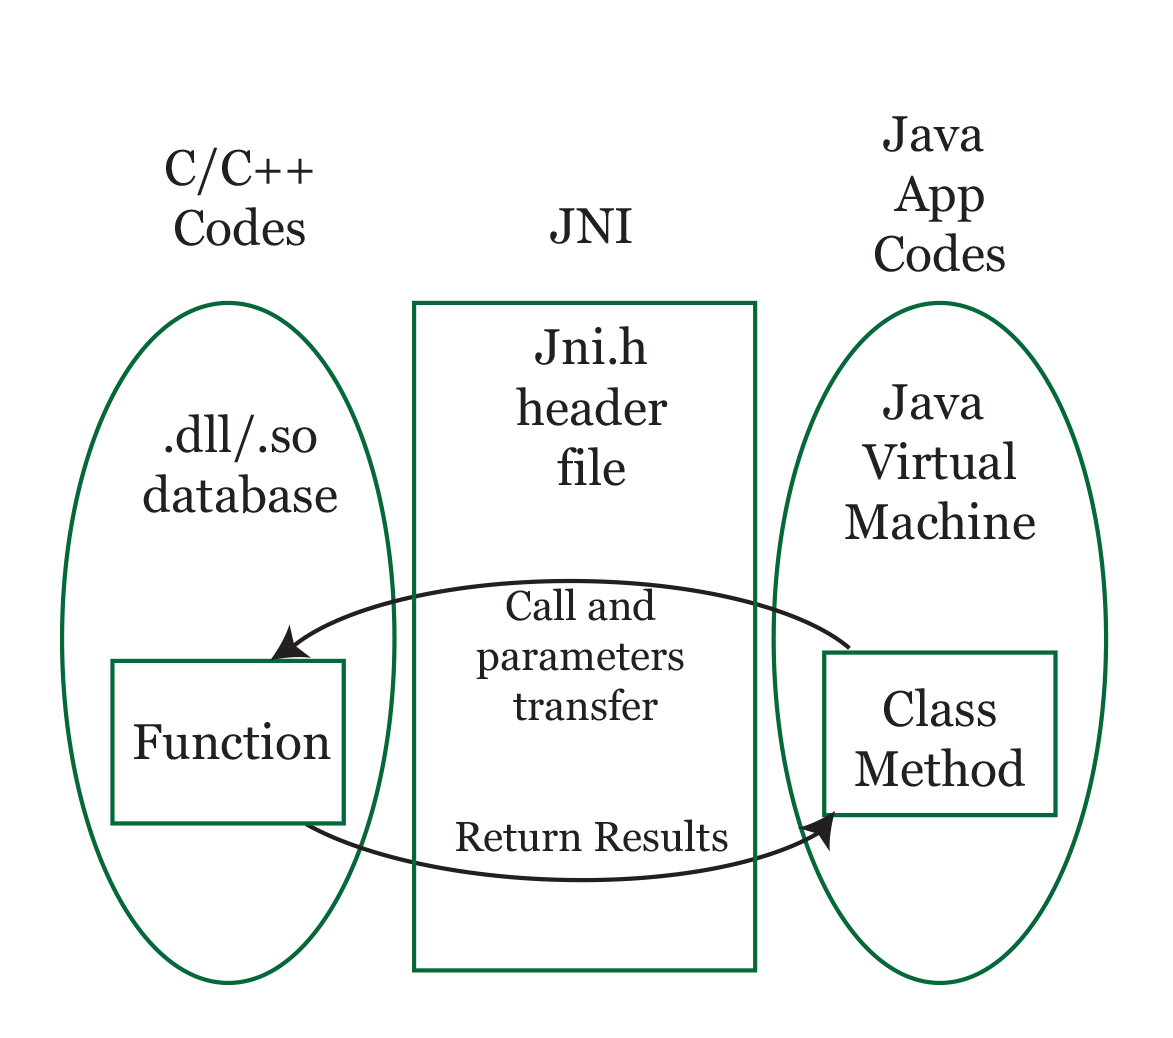
\includegraphics[keepaspectratio,scale=0.3]{JNI.png}
\end{figure}


\section{User Interface}

\par
The Android User Interface is programmed in Java and only one thread can refresh the User Interface (UI thread).

\par
There are only two goals in the User Interface: should be as simple as possible and should be able to allow progressive ray tracing, which means, refreshing the image while it is being rendered.

\par
In order to allow progressive ray tracing, it was used a pool of one thread called Render Task thread that every 250 ms wakes up the thread and updates the strings used in the text view.
Before it finishes, it publishes the progress on the UI thread.
Then the UI thread wakes up and updates the text view.

\begin{figure}[H]
	\centering
	\caption{Execution flow of UI thread and Render Task thread.}
	\label{Execution flow of UI thread and Render Task thread}
	\includegraphics[keepaspectratio,scale=0.5]{UI_thread.png}
\end{figure}

\section{Programming decisions}

\par
The main goal of programming this library in a object oriented manner is to have a library with relatively good performance and with a maintainable code.

\par
Besides that, it was used the smart pointers available in the C++ standard library.
The smart pointer used was the unique pointer, as this was enough for this project and also because it is the smart pointer with best performance.
This smart pointer automatically free the resources it contains.
This greatly reduces the chance of the programmer to forget to free a resource or trying to free it multiple times.
Of course this comes with a little performance cost of about 1\% to 5\% relatively to the manual resource management by the programmer.
But for this project, some extra code correctness is more important than more performance.

\subsection{Challenges}

\par
Developing applications for mobile devices have different challenges compared with the traditional personal computer hardware.

\par
The Android User Interface has some particularities like only one thread can modify the UI, and is usually called the UI thread.

\par
The size of RAM available for executing applications is typically smaller.
In the 2010s the most expensive mobile devices had only about 512MB of RAM, and nowadays most of them have more than 4GB.
But, still, comparing them with personal computers which typically have 16GB it is a big difference.
This can make a big impact in the maximum number of vertices that a scene can have in the ray tracer.

\par
And the CPU microarchitecture is generally simpler and with smaller computational power.
Also the Operating System (OS) is shaped for the mobile world, making a lot of restrictions in the performance of the applications in order to save battery.
The amount of main memory available for the applications can also be affected by the OS.

\par
Other challenges are related with the communication mechanism between the SDK and the NDK, because two different languages environments need to "communicate" in runtime (GUI in Java and the library in C++).
This involves learning how to use the Java Native Interface (JNI), so that the native code can send and receive information from Java Virtual Machine (JVM).

\par
Because ray tracing may involve rendering complex scenes, placing all this information in the main memory may not be possible, and so this memory management can be a worthy challenge.

\section{Comparison with Android CPU Raytracer (\cite{Android_CPU_Raytracer})}

\par
Comparison ...